\documentclass[]{article}

% Imported Packages
%------------------------------------------------------------------------------
\usepackage{amssymb}
\usepackage{amstext}
\usepackage{amsthm}
\usepackage{amsmath}
\usepackage{enumerate}
\usepackage{float}
\usepackage{fancyhdr}
\usepackage[margin=1in]{geometry}
\usepackage{graphicx}
\usepackage{extarrows}
\usepackage{setspace}
\usepackage{indentfirst}
\usepackage{makecell}
%------------------------------------------------------------------------------

% Header and Footer
%------------------------------------------------------------------------------
\pagestyle{plain}  
\renewcommand\headrulewidth{0.4pt}                                      
\renewcommand\footrulewidth{0.4pt}                                    
%------------------------------------------------------------------------------

% Title Details
%------------------------------------------------------------------------------
\title{Deliverable \#2}
\author{SE 3A04: Software Design II -- Large System Design}
\date{\today}                               
%------------------------------------------------------------------------------

% Document
%------------------------------------------------------------------------------
\begin{document}

\maketitle	

\section{Introduction}
\label{sec:introduction}
% Begin Section

The following document will give an overall description of the components of the project.

\subsection{Purpose}
% Begin Purpose
This is a high-level design document created for blocking out the components of the system. The components will be guided by the business events and describes what each component will be doing. The intended audience for this document is software engineers designing this system.
% End Purpose

\subsection{System Description}
\label{sub:system_description}
% Begin SubSection
Ship Wreck is a single-player game. It has one core goal, which can be achieved by playing five different mini-games. The ship will be wrecked if its health reaches or goes below 0. Since completing mini-games can prevent the health of this ship from reaching 0, players need to complete as many mini-games as provided to ensure that the ship can reach its destination safely.
% End SubSection

\subsection{Overview}
\label{sub:overview}
% Begin SubSection
The rest of this document will be organized into sections describing the analysis class diagram, the architectural design and CRC cards. These will describe what the software will be expected to do.
% End SubSection

% End Section

\section{Analysis Class Diagram}
\label{sec:analysis_class_diagram}
% Begin Section
\begin{figure}[H]
    \centering
    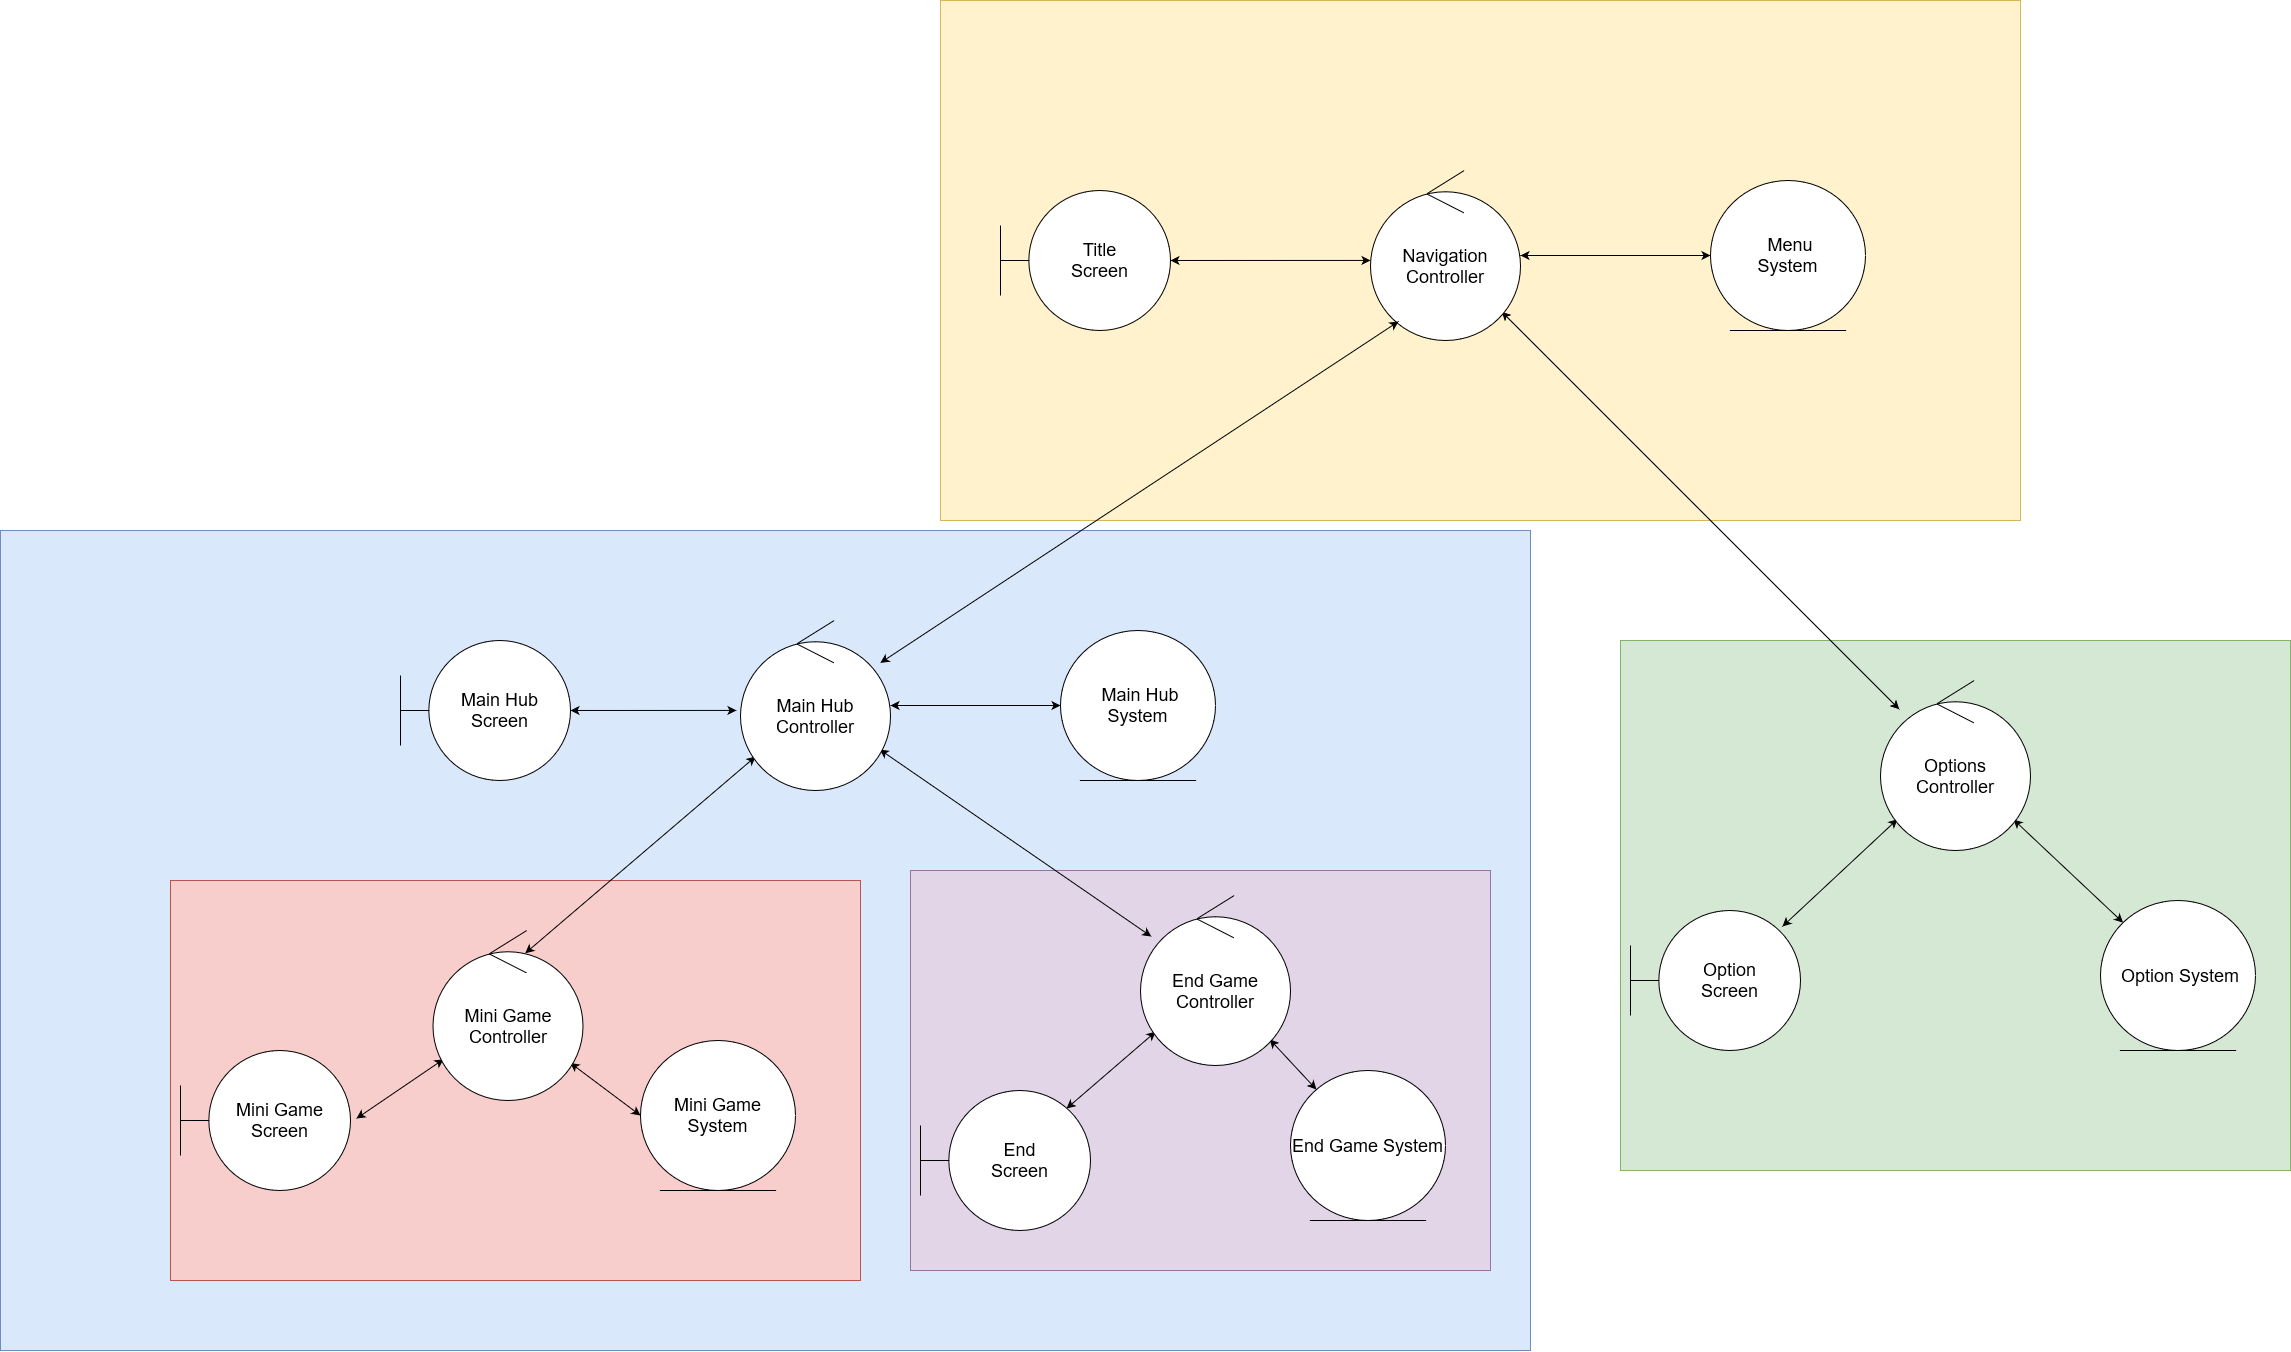
\includegraphics[width=1.10\textwidth]{figures/ACD.png}
    \caption{Block diagram of the project}
    \label{fig:acd}
\end{figure}
% End Section


\section{Architectural Design}
\label{sec:architectural_design}
% Begin Section

\subsection{System Architecture}
\label{sub:system_architecture}
% Begin SubSection
The presentation-abstraction-control (PAC) architecture is ideal for the system. As a game is being designed for this project, the focus is on a player's interaction with the game and how the game can process constant input data effectively.

The PAC architecture offers a separation of concerns. A hierarchy of agents is introduced, each of which has a presentation, controller and abstraction component.

The presentation component deals with displaying data in a way that is intuitive for the user. The abstraction component would contain the data necessary. The controller processes user input and manipulates the abstraction component, and communicates with other controllers above and below it in the hierarchy.

Through this separation of concerns, the PAC architecture provides modularization and independence among agents. Changes in one component will not affect other components, as each component is concerned with its own set of activities, determined by the abstraction component.

All activities pertaining to a specific agent will be done in that agent. If an activity must be done with a different agent, communication will be conducted through the agents' controller component. This allows for any bugs pertaining to a component to be detected and fixed quickly. 
% End SubSection

\subsection{Subsystems}
\label{sub:subsystems}
% Begin SubSection
The core component and the removable mini-parts would be the subsystems of the PAC architecture. 

As shown in the analysis case diagram, the core component and each mini-part will include its own PAC structure. This will allow the project to create barriers and organize the system into a hierarchy. In addition, the PAC architecture defines a succinct way to facilitate communication among these subsystems, as it will define a structure in the form of a hierarchy of cooperating agents, communicating solely through controllers.
% End Subsection

% End Section
	
\section{Class Responsibility Collaboration (CRC) Cards}
\label{sec:class_responsibility_collaboration_crc_cards}
% Begin Section

\begin{table}[H]
	\centering
	\begin{tabular}{|p{5cm}|p{5cm}|}
	\hline 
	\multicolumn{2}{|l|}{\textbf{Class Name: Options Controller}} \\
	\hline
	\textbf{Responsibility:} & \textbf{Collaborators:} \\
	\hline
	\makecell[l]{
	Receive options\\
	Store options in system\\
	Confirm options have been saved\\ 
	Facilitate exit navigation
	} & \makecell[c]{Options Screen}\\
	\hline
	\end{tabular}
\end{table}	


\begin{table}[H]
	\centering
	\begin{tabular}{|p{5cm}|p{5cm}|}
	\hline 
	\multicolumn{2}{|l|}{\textbf{Class Name: Option System}} \\
	\hline
	\textbf{Responsibility:} & \textbf{Collaborators:} \\
	\hline
	\makecell[l]{
	Know difficulty level\\
	Know character selection\\
	Know in-game volume level\\
	Know mute state
	} & \makecell[c]{
	% None
	}\\
	\hline
	\end{tabular}
\end{table}	

\begin{table}[H]
	\centering
	\begin{tabular}{|p{5cm}|p{5cm}|}
	\hline 
	\multicolumn{2}{|l|}{\textbf{Class Name: Option Screen}} \\
	\hline
	\textbf{Responsibility:} & \textbf{Collaborators:} \\
	\hline
	\makecell[l]{
	Display user's options\\
	Allow input of options\\
	Allow saving of new options\\
	Allow exit from screen
	} & \makecell[c]{Options Controller}\\
	\hline
	\end{tabular}
\end{table}	

\begin{table}[H]
	\centering
	\begin{tabular}{|p{5cm}|p{5cm}|}
	\hline 
	\multicolumn{2}{|l|}{\textbf{Class Name: Navigation Controller}} \\
	\hline
	\textbf{Responsibility:} & \textbf{Collaborators:} \\
	\hline
	\makecell[l]{
	Facilitate transfer to main hub\\
	Facilitate transfer to settings \\
	Check high-score\\
	Receive settings\\
	} & \makecell[c]{Title Screen\\Main Hub Controller\\Options Controller}\\
	\hline
	\end{tabular}
\end{table}	

\begin{table}[H]
	\centering
	\begin{tabular}{|p{5cm}|p{5cm}|}
	\hline 
	\multicolumn{2}{|l|}{\textbf{Class Name: Menu System}} \\
	\hline
	\textbf{Responsibility:} & \textbf{Collaborators:} \\
	\hline
	\makecell[l]{Know player high score} & \makecell[c]{
	% None
	}\\
	\hline
	\end{tabular}
\end{table}	

\begin{table}[H]
	\centering
	\begin{tabular}{|p{5cm}|p{5cm}|}
	\hline 
	\multicolumn{2}{|l|}{\textbf{Class Name: Title Screen}} \\
	\hline
	\textbf{Responsibility:} & \textbf{Collaborators:} \\
	\hline
	\makecell[l]{
	Presents start game button\\
	Presents options button\\
	Allows input of start game\\
	Allows input to go to options\\
	\\
	} & \makecell[c]{Navigation Controller}\\
	\hline
	\end{tabular}
\end{table}	

\begin{table}[H]
	\centering
	\begin{tabular}{|p{5cm}|p{5cm}|}
	\hline 
	\multicolumn{2}{|l|}{\textbf{Class Name: Main Hub Controller}} \\
	\hline
	\textbf{Responsibility:} & \textbf{Collaborators:} \\
	\hline
	\makecell[l]{Save mini-game status\\
	            Facilitate transfer to mini-game\\
            	Check win/lose status\\ Determine longest survival time} & 
    \makecell[c]{Main Hub Screen\\Mini Game Controller\\End Game Controller\\Navigation Controller}\\
	\hline
	\end{tabular}
\end{table}	

\begin{table}[H]
	\centering
	\begin{tabular}{|p{5cm}|p{5cm}|}
	\hline 
	\multicolumn{2}{|l|}{\textbf{Class Name: Main Hub System}} \\
	\hline
	\textbf{Responsibility:} & \textbf{Collaborators:} \\
	\hline
	\makecell[l]{Know win/lose data\\ Know remaining mini-games\\ Know time left} & \makecell[c]{
% 	None
	}\\
	\hline
	\end{tabular}
\end{table}	

\begin{table}[H]
	\centering
	\begin{tabular}{|p{5cm}|p{5cm}|}
	\hline 
	\multicolumn{2}{|l|}{\textbf{Class Name: Main Hub Screen}} \\
	\hline
	\textbf{Responsibility:} & \textbf{Collaborators:} \\
	\hline
	\makecell[l]{Display remaining mini-games\\Receive user movement inputs\\Display time left} & \makecell[c]{Main Hub Controller}\\
	\hline
	\end{tabular}
\end{table}	

\begin{table}[H]
	\centering
	\begin{tabular}{|p{5cm}|p{5cm}|}
	\hline 
	\multicolumn{2}{|l|}{\textbf{Class Name: Mini Game Controller}} \\
	\hline
	\textbf{Responsibility:} & \textbf{Collaborators:} \\
	\hline
	\makecell[l]{Receive mini-game name\\Process user inputs\\Start mini-game\\Set mini-game's difficulty level} & \makecell[c]{Main Hub Controller\\Mini Game Screen}\\
	\hline
	\end{tabular}
\end{table}	

\begin{table}[H]
	\centering
	\begin{tabular}{|p{5cm}|p{5cm}|}
	\hline 
	\multicolumn{2}{|l|}{\textbf{Class Name: Mini Game Screen}} \\
	\hline
	\textbf{Responsibility:} & \textbf{Collaborators:} \\
	\hline
	

	\makecell[l]{Receive user inputs\\ Display mini-game target and\\current score\\ Display time left\\ Display mini-game pass/fail\\status} & \makecell[c]{Mini Game Controller}\\
	\hline
	\end{tabular}
\end{table}	

\begin{table}[H]
	\centering
	\begin{tabular}{|p{5cm}|p{5cm}|}
	\hline 
	\multicolumn{2}{|l|}{\textbf{Class Name: Mini Game System}} \\
	\hline
	\textbf{Responsibility:} & \textbf{Collaborators:} \\
	\hline
	\makecell[l]{Know mini-game pass/fail status\\Know mini-game's name\\Know gained score\\Know target score\\Know time left\\Know the mini-game's difficulty\\level} & \makecell[c]{
% 	None
	}\\
	\hline
	\end{tabular}
\end{table}	

\begin{table}[H]
	\centering
	\begin{tabular}{|p{5cm}|p{5cm}|}
	\hline 
	\multicolumn{2}{|l|}{\textbf{Class Name: End Game Controller}} \\
	\hline
	\textbf{Responsibility:} & \textbf{Collaborators:} \\
	\hline
	\makecell[l]{Receive current game score\\Receive high score\\Receive time survived in current \\ game \\Receive longest survival time\\Determine win/lose status} & \makecell[c]{End Game Screen\\Main Hub Controller}\\
	\hline
	\end{tabular}
\end{table}	

\begin{table}[H]
	\centering
	\begin{tabular}{|p{5cm}|p{5cm}|}
	\hline 
	\multicolumn{2}{|l|}{\textbf{Class Name: End Game Screen}} \\
	\hline
	\textbf{Responsibility:} & \textbf{Collaborators:} \\
	\hline
	\makecell[l]{Display win/lose status\\Display current game score\\Display high score\\Display longest survival time} & \makecell[c]{End Game Controller}\\
	\hline
	\end{tabular}
\end{table}	

\begin{table}[H]
	\centering
	\begin{tabular}{|p{5cm}|p{5cm}|}
	\hline 
	\multicolumn{2}{|l|}{\textbf{Class Name: End Game System}} \\
	\hline
	\textbf{Responsibility:} & \textbf{Collaborators:} \\
	\hline
	\makecell[l]{Know win/lose status} & \makecell[c]{
	%None
	}\\
	\hline
	\end{tabular}
\end{table}	

\newpage
\appendix
\section{Division of Labour}
\label{sec:division_of_labour}

Include a Division of Labour sheet which indicates the contributions of each team member. This sheet must be signed by all team members.

\begin{table}[h]
    \centering
    \begin{tabular}{|c|c|c|}
    \hline
        \textbf{Name} & \textbf{Contributed Part} & \textbf{Signature} \\
        \hline
        Benson & 
        Section 1, 3 \& 4 & 
\includegraphics[width=0.3\textwidth]{signatures/bensonsignature.JPG}\\
        \hline
        Graeme & 
        Section 2 \& 4 & 
\includegraphics[width=0.25\textwidth]{signatures/graeme_signature.png} \\
        \hline
        Jiawei & 
        Section 1, 3 \& 4 & 
\includegraphics[width=0.3\textwidth]{signatures/Signature_Jiawei.PNG}\\
        \hline
        Nick & 
        Section 2 \& 4 & 
\includegraphics[width=0.3\textwidth]{signatures/nick signature.PNG} \\
        \hline
        Rupinder & 
        Section 1, 3 \& 4 & 
\includegraphics[width=0.3\textwidth]{signatures/Rupinder Signature.png}\\
        \hline
    \end{tabular}
    \caption{Division of Labour}
    \label{tab:my_label}
\end{table}


\newpage
\section*{IMPORTANT NOTES}
\begin{itemize}
%	\item You do \underline{NOT} need to provide a text explanation of each diagram; the diagram should speak for itself
	\item Please document any non-standard notations that you may have used
	\begin{itemize}
		\item \emph{Rule of Thumb}: if you feel there is any doubt surrounding the meaning of your notations, document them
	\end{itemize}
	\item Some diagrams may be difficult to fit into one page
	\begin{itemize}
		\item It is OK if the text is small but please ensure that it is readable when printed
		\item If you need to break a diagram onto multiple pages, please adopt a system of doing so and thoroughly explain how it can be reconnected from one page to the next; if you are unsure about this, please ask about it
	\end{itemize}
	\item If you do \underline{NOT} have a Division of Labour sheet, your deliverable will \underline{NOT} be marked
\end{itemize}


\end{document}
%------------------------------------------------------------------------------